\begin{chapter}{Cloud services}
    \label{chap:cloud_services}

    In the early days of the web, anyone who wanted to build a web application had
    to buy and maintain the physical hardware required to run a server, which was
    a cumbersome process to undertake, especially for small businesses
    \cite{what_is_sls_cloudflare}.
    Then came a new paradigm for the provisioning of computing infrastructure, named
    Cloud Computing, and defined as:

    \enquote*{%
        Clouds are a large pool of easily usable and accessible virtualized resources
        (such as hardware, development platforms and/or services). These resources
        can be dynamically reconfigured to adjust to a variable load (scale), allowing
        also for an optimum resource utilization. This pool of resources is typically
        exploited by a pay-per-use model in which guarantees are offered by the
        Infrastructure Provider by means of customized SLAs.%
    } \cite{cloud_computing_definition}

    \begin{figure}
        \centering
        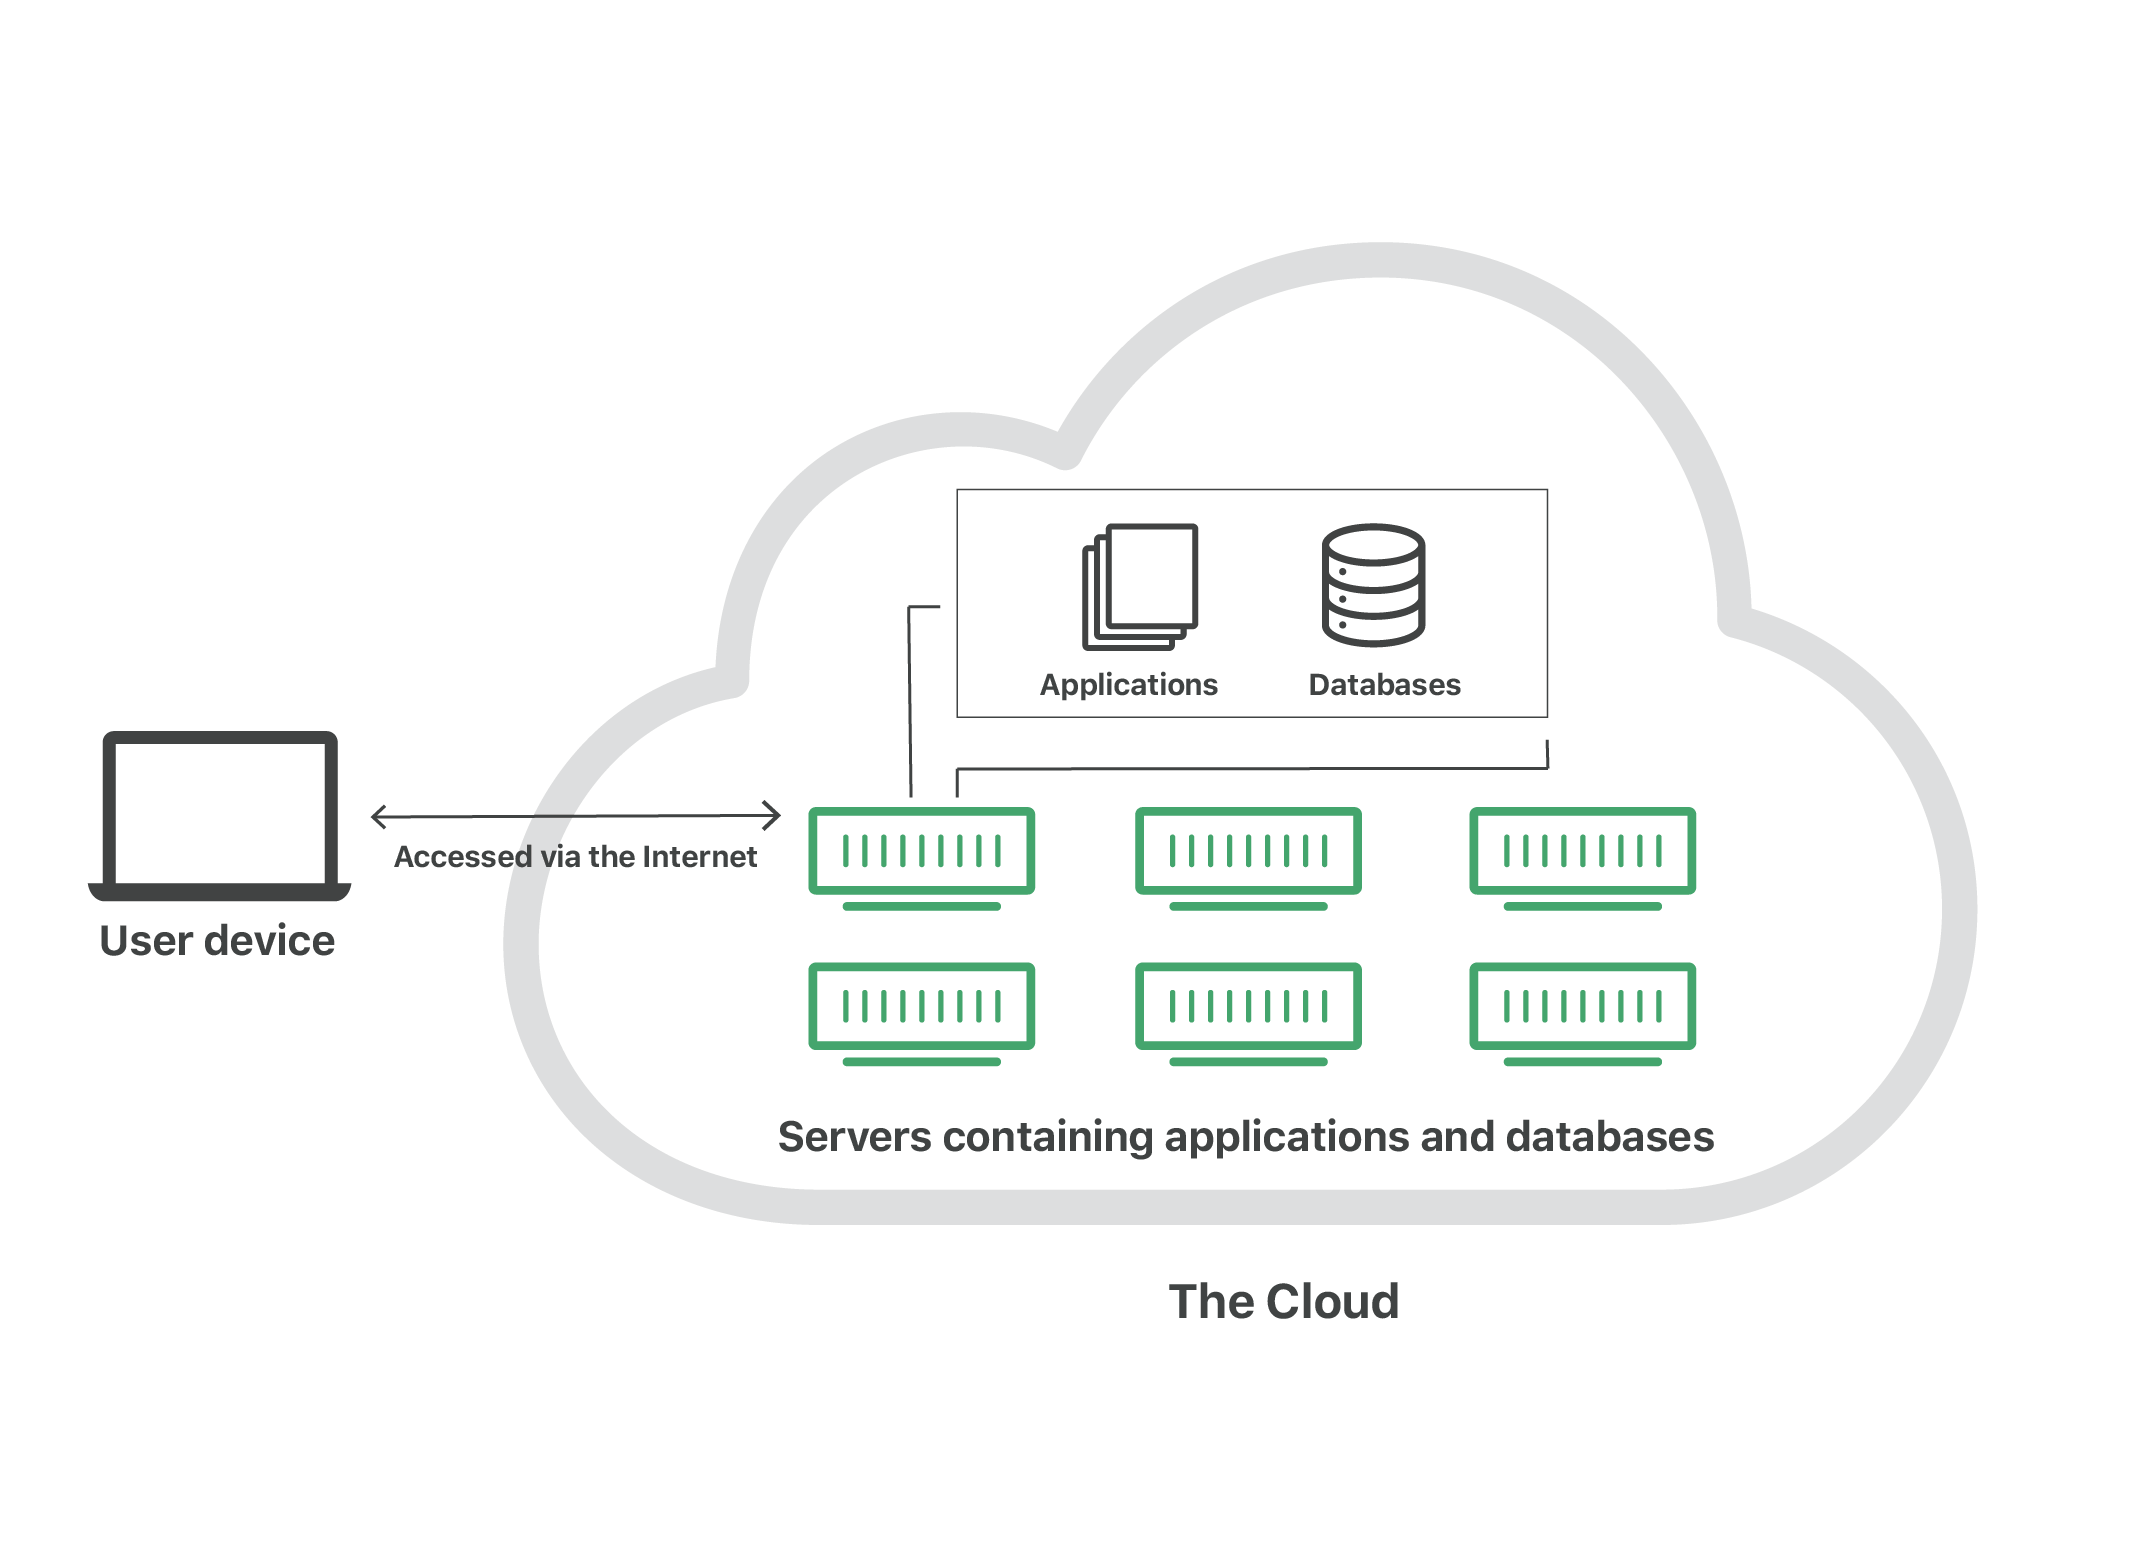
\includegraphics[width=10cm]{source/images/what-is-the-cloud.png}
        \caption{Representation of the cloud}
    \end{figure}

    Cloud Computing is possible because of a technology called virtualization, which
    allows the creation of a simulated computer, named virtual machine, that behaves
    as if it were a physical computer with its own hardware. When properly implemented,
    this approach allows having a more efficient use of the physical hardware, as
    each computer is able to run many virtual machines at once.
    Despites the many benefits, using virtual machines still requires manual server
    administration, as each one simulate a full system, including the operating
    system and the underlying kernel.

    The next technological step has been containerization, which gave the possibility
    of packing an application and all its dependencies, such as system libraries
    and system settings into a single entity called Container. With this approach
    a single physical machine, including the kernel, is shared by a multitude of
    containers. The main advantages that containerization offers, with respect to
    virtual machines are \cite{what_is_the_cloud}:
    \begin{itemize}
        \item Portability: once the application is packed into a container it can
            be run on any host supporting that technology.
        \item Control and flexibility.
        \item Faster deploy.
        \item Less server administration.
    \end{itemize}
    With this premises about the cloud and its infrastructure is possible to outline
    the main models that have emerged in the context of cloud computing.

    \section{Cloud computing models}
    Among the various types of cloud computing architectures have emerged three
    main models, which are: Infrastructure as a Service, Platform as a Service and
    Software as a Service. Each model is characterized by an increasing level of
    abstraction regarding the underlying infrastructure.

    \begin{figure}
        \centering
        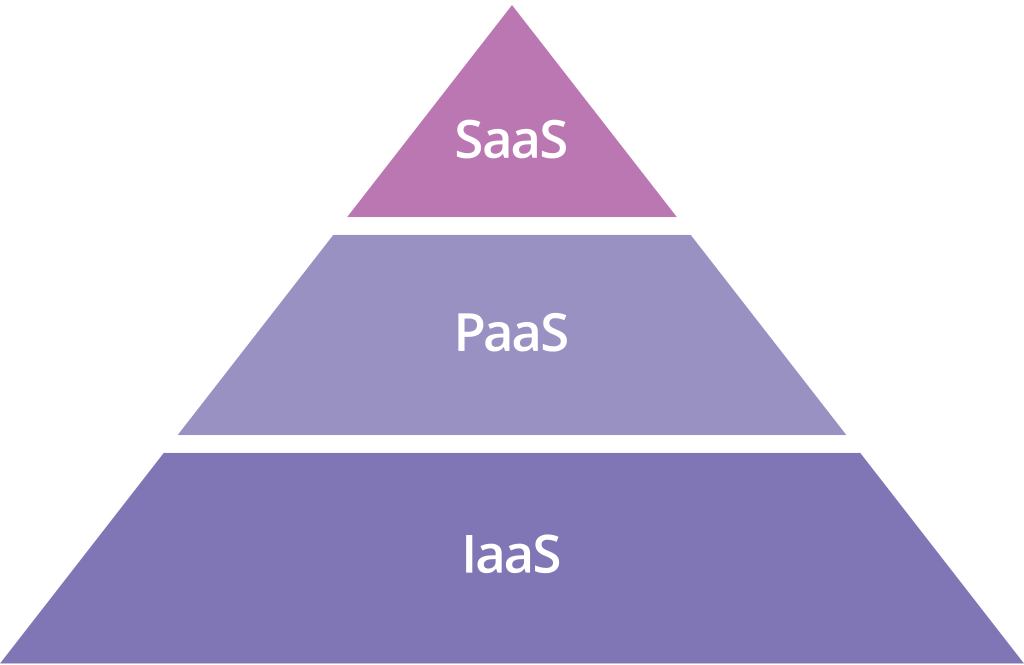
\includegraphics[height=3cm]{source/images/saas-paas-iaas-cloud-pyramid.png}
        \caption{IaaS, PaaS, SaaS Pyramid}
        \label{fig:cloud_computing_pyramid}
    \end{figure}

    \subsection{Infrastructure as a Service (IaaS)}
    Infrastructure refers to the computers and servers than run code and store data.
    A vendor hosts the infrastructure in data centers, referred to as the cloud,
    while customers access it over the Internet. This eliminates the need for customers
    to own and manage the physical infrastructure, so they can build and host web
    applications, store data or perform any kind of computing with a lot more flexibility.
    An advantage of this approach is scalability, as customers can add new servers
    on demand, every time the business needs to scale up, and the same apply also
    if the resources are not needed anymore. Essentially physical servers purchasing,
    installing, maintenance and updating operations are outsourced to the cloud
    provider, so customers can spend fewer resources on that and focus more on business
    operations, thus leading to a faster time to market. The main drawback of this
    approach is the cost effectiveness, as businesses needs to over-purchase resources
    to handle usage spikes, this leads to wasted resources \cite{iaas}.

    \subsection{Platform as a Service (PaaS)}
    This model simplify web development, from a developer perspective, as they can
    rely on the cloud provider for a series of services, which are vendor dependent.
    However some of them can be defined as core PaaS services, and those are: development
    tools, middleware, operating systems, database management, and infrastructure.
    PaaS can be accessed over any internet connection, so developers can work on
    the application from anywhere in the world and build it completely on the browser.
    This kind of simplification comes at the cost of less control over the development
    environment \cite{paas}. An example of this kind of services is Google's
    \href{https://cloud.google.com/appengine}{App Engine}.

    \smallskip
    Another model has recently been added to the three main cloud computing models,
    named Backend as a Service (Baas). This model stands, with some differences,
    at the same level of PaaS, and it's suited especially for web and mobile backend
    development. As with PaaS, BaaS also makes the underlying server infrastructure
    transparent from the developer point of view, and also provides the latter with
    api and sdk that allow the integration of the required backend functionalities.
    The main functionalities already implemented by BaaS are: database management,
    cloud storage, user authentication, push notifications, remote updating and hosting.
    Thanks to these functionalities there may be a greater focus on frontend or mobile
    development.
    In conclusion BaaS provides more functionalities with respect to the PaaS model,
    while the latter provides more flexibility.

    \subsection{Software as a Service (SaaS)}
    In this model the abstraction from the underlying infrastructure is maximized.
    The vendor makes available a fully built cloud application to customers, through
    a subscription contract, so rather than purchasing the resource once there is
    a periodic fee. The main advantages of this model are: access from anywhere,
    no need for updates or installations, scalability, as it's managed by the SaaS
    provider, cost savings.
    However there are also main disadvantages, that makes this solution not suitable
    in some cases: developers have no control over the vendor software, the business
    may become dependent on the SaaS provider (vendor lock-in), no direct control
    over security, this may be an issue especially for large companies \cite{saas}.

    \begin{figure}
        \centering
        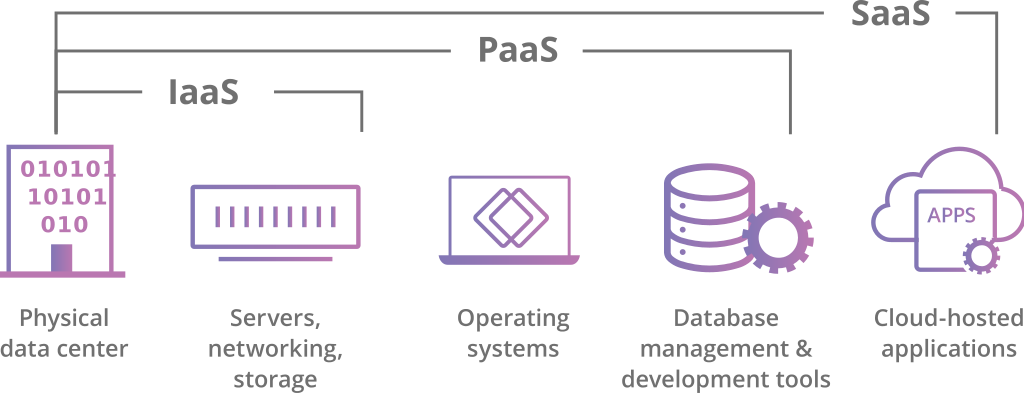
\includegraphics[width=\linewidth]{source/images/saas-paas-iaas-diagram.png}
        \caption{IaaS, PaaS, SaaS diagram}
        \label{fig:cloud_computing_architectures}
    \end{figure}

    \section{Serverless paradigm}
    The downsides of the previously described approaches varies from the control on the
    infrastructure and on the software, to scalability problems, to end with cost
    and resources utilization effectiveness.
    Aiming to solve these problems, the major providers started investing on a new
    cloud computing model, named Function as a Service (FaaS) and based on the
    serverless paradigm.
    Such a paradigm is based on providing backend services on an as-used basis, with
    the cloud provider allowing to develop and deploy small piece of code without
    the developer having to deal with the underlying infrastructure.
    So despite the terminology, serverless does not mean without servers, as they are
    of course still required, but they are transparent to developers, which can focus
    on smaller pieces of code.
    With this model, rather than over purchase the resources, to ensure correct
    functionality in all workload situations, as happens in the IaaS model, the vendor
    charges for the actual usage, as the service is auto-scaling. Thanks to this approach
    consumer costs will be fine grained as shown in \ref{fig:serverless_benefits}.

    \begin{figure}
        \centering
        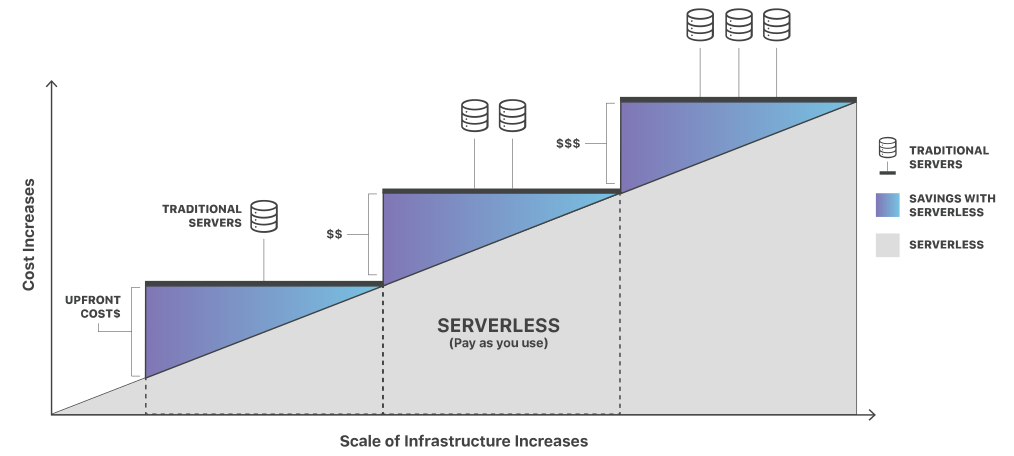
\includegraphics[width=\linewidth]{source/images/benefits-of-serverless.png}
        \caption{Cost Benefits of Serverless}
        \label{fig:serverless_benefits}
    \end{figure}

    Being the underlying infrastructure transparent for the developer, you get the advantage
    of a simpler software development process, and this advantage characterize also
    the PaaS model. Furthermore, being the service auto-scaling, is possible to obtain
    a virtually unlimited scaling capacity, as it happens in the IaaS model, where the
    limit is the cloud provider availability.

    An implementation of the serverless paradigm is the cloud model named Function
    as a Service (FaaS), which allows developers to write and update pieces of code
    on the fly, typically a single function.
    Such code is then executed in response to an event, usually an api call, but other
    options are possible, so it executed regardless of the events, and this lead to
    the previously described benefit regarding scalability and cost effectiveness.
    Furthermore, through this model turns out to be more efficient to implement web
    applications using the modular approach of the micro services architecture
    (\ref{fig:monolithic_to_microservices}), since the code is organized as a set of
    independent functions from the beginning.

    \begin{figure}
        \centering
        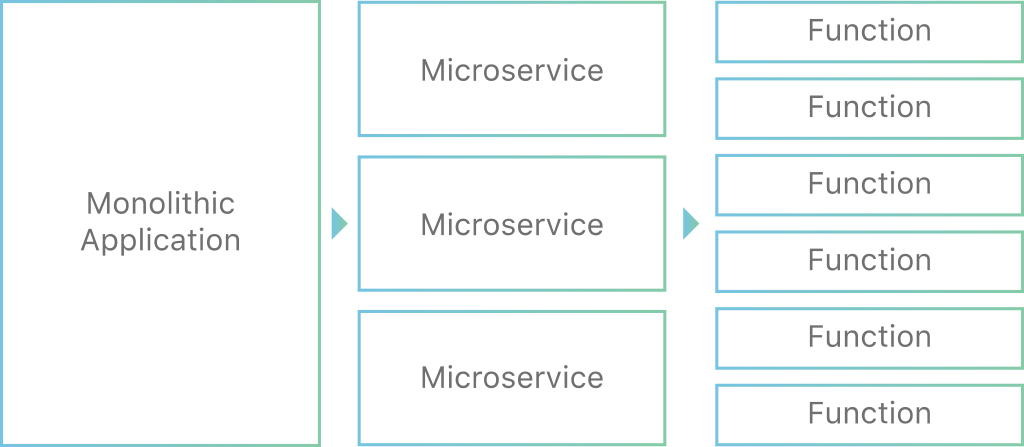
\includegraphics[width=\linewidth]{source/images/monolithic-application-microservice-faas.png}
        \caption{Monolithic to Micro services application}
        \label{fig:monolithic_to_microservices}
    \end{figure}

    So the main advantages of the FaaS model are: improved developer speed, built-in
    scalability and cost efficiency. As each approach, there are also drawbacks, in
    this case developers have less control on the system, and an increased complexity when it
    comes to test the application in a local environment.

    The first cloud provider to move into the FaaS director has been Amazon, with the
    introduction of aws lambda in 2014, followed by microsoft and google, with
    azure function and cloud function respectively in 2016.

    \section{Serverless Framework}
    \label{sec:serverless_framework}
    Shortly after the release of the service Aws lambda functions, has been introduced,
    in 2015, the Serverless framework, with the main objective of making development,
    deploy and troubleshoot serverless applications with the least possible overhead.
    The framework consists of an open source Command Line Interface and a hosted
    dashboard, that combined provide developers with serverless application lifecycle
    management. Serverless supports all runtime provided by Aws, corresponding to
    the most popular programming languages such as: Node.js, Python, Ruby, Java,
    Go, .Net, and others are on development.

    Although the serverless framework, given the number of cloud providers supported,
    aim to be platform agnostic, the following examples will be based on the Aws
    provider and on the Node.js programming language.

    The main work units of the framework, according to the FaaS model, are the functions.
    Each function is responsible for a single job, and although is possible to perform
    multiple tasks using a single function, it's not recommended as stated by the
    design principle Separation of concerns \cite{separation_of_concerns}.
    Each function is executed only when triggered by and Event, which can be of different
    type, such as: http api request, scheduled execution and image or file upload.
    Once the developer has defined the function and the events associated to it,
    the framework take care of creating the necessary resources on the provider platform.

    The framework introduces the concept of Services as unit of organization. Each
    service has one or more functions associated to it and an application can then
    be composed by multiple services. This structure reflects the modular approach
    of the micro services architecture described previously. Finally various applications
    are grouped under an organization (\ref{fig:sls_resource_scheme})

    \begin{figure}
        \centering
        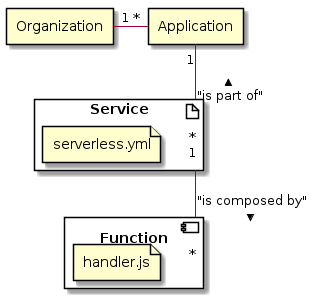
\includegraphics[width=6.5cm]{source/diagrams/serverless_app_service.png}
        \caption{Serverless framework resources scheme}
        \label{fig:sls_resource_scheme}
    \end{figure}

    A service is described by a file, located at the root directory of the project,
    and composed in the format \href{https://yaml.org/}{Yaml} or Json.
    Below is a simple serverless.yml file (listing \ref{lst:simple_sls_yml}), it
    defines the service users, which contains just a function, responsible of creating
    a user. The handler field specify the path to the function code, in this case
    the framework will search for a handler.js file, exporting a usersCreate function,
    as show on listing \ref{lst:handler_fun}.

    \bigskip
    \begin{code}[caption=Simple serverless.yml file, label={lst:simple_sls_yml}]
org: my-company-org
app: chat-app
service: users
provider:
  name: aws
  runtime: nodejs12.x
functions:
  usersCreate:
    handler: handler.usersCreate
    events:
      - http: post users/create
    \end{code}

    \begin{code}[caption=Simple handler function, label={lst:handler_fun}]
async function usersCreate(event, context) {
  const user = {
    name: 'sample_name',
    surname: 'sample_surname'
  }
  await mockDb.createUser(user)
  return {
    statusCode: 200,
    body: JSON.stringify({user})
  }
}
    \end{code}

    \begin{figure}
        \begin{minipage}{\linewidth}
            \dirtree{%
                .1 ./.
                .2 handler.js.
                .2 serverless.yml.
            }
        \end{minipage}
        \caption{Simple Serverless project structure}
        \label{fig:sls_project_structure}
    \end{figure}

    Serverless is flexible and does not force a fixed structure of the project, that
    task is up to the developer.
    Defined that structure, the service can be deployed using the Serverless CLI, on
    the chosen provider, as shown on listing \ref{lst:sls_deploy}.

    \bigskip
    \begin{code}[caption=Deploy command, label={lst:sls_deploy}]
$ serverless deploy
Serverless: Stack update finished...
Service Information
service: users
stage: dev
region: us-east-1
stack: users-dev
resources: 12
api keys:
  None
endpoints:
  POST - https://.../dev/users/create
functions:
  usersCreate: users-dev-usersCreate
layers:
  None
    \end{code}

    The deploy command creates the necessary aws resources, in this case they are:
    a lambda function corresponding to the usersCreate function and an api gateway to
    handle http requests.
    It is then possible to test the newly created resource by making requests to the
    url returned by the CLI, specifying the resource path /users/create.
    It is possible to invoke online functions also directly from the CLI,
    specifying the identifier of the function used in the serverless.yml file, as shown
    on listing \ref{lst:sls_invoke}

    \bigskip
    \begin{code}[caption=Invoke command, label={lst:sls_invoke}]
$ serverless invoke -f usersCreate
{
    "statusCode": 200,
    "body": "{\"user\":{\"name\":\"sample_name\", ...}}"
}
    \end{code}

    The development and deploy process shown for a service with a single function
    remains the same as the service complexity grows, in particular it is possible to
    modify and deploy a single function at a time, since each function has its own
    resource associated.
    This process gets along with the previously described micro services architecture.

    \subsection{Advantages}
    The main advantages of using the Serverless framework are:
    \begin{itemize}
        \item Provider agnostic: the framework aims to be independent from the chosen
            cloud provider, thus avoiding vendor lock-in. In practice this feature is
            not achieved completely, as the configuration file serverless.yml may be
            different across providers. However the main structure remains the same,
            and that simplify providers migration.
        \item Simplified development: the CLI commands simplify the development process,
            from the deploy from the testing of the deployed functions.
        \item Extensible: is possible to develop plugins that integrate with the
            CLI commands lifecycle, increasing their functionalities.
        \item Dashboard: the hosted dashboard allow monitoring and tracing of the
            deployed functions and services.
    \end{itemize}

    \subsection{Disadvantages}
    \label{subsec:sls_disadvantage}
    The main advantages of using the Serverless framework and the Serverless paradigm are:
    \begin{itemize}
        \item Compilation of the configuration file may become tedious as the project grows.
        \item The framework is extremely flexible regarding the project structure and
            that is an advantage, however this can be also a drawback as it's up to the
            developer to find a suitable structure, and this means less time spent on
            business related tasks.
        \item Unit testing: it is possible to test a deployed function easily, however
            for big projects, where it's necessary to test a lot of functions, this may
            become cumbersome.
        \item Resource threshold: for projects created with Aws, a single
            serverless.yml file may create up to 200 resources, and if exceeded
            the deploy operation fails. Since each function is responsible for the
            creation of about 10 resources, is very easy to exceed this limit.
            The only solution so solve this problem is to split the functions across
            multiple services, hence different serverless.yml configuration files.
        \item Cold start: inherent overhead of the current implementation of the
            serverless paradigm. Since each function is executed only in response to
            an event, a certain amount of time is required for resources initialization.
    \end{itemize}

    \section{Conclusions}
    Each cloud model presented has its own strength and drawbacks, depending on the
    needs of the wanted goal. Favouring as selection criteria, solutions that present
    major advantages in terms of scalability, cost efficiency and speed of development,
    has been decided to favour the Serverless option.
    The main cloud providers offering this kind of service, as previously stated,
    are: Aws, with its Lambda service, Microsoft, with Azure Functions, and Google,
    with Cloud Functions. Each provider offer different configurations, with different
    pricing, based on memory, CPU, and execution time as parameters, as shown on
    \ref{table:cloud_providers_offer}.
    In the literature there are several documents comparing the various services
    side by side exhaustively \cite{sls_providers_comparison}.
    For the project subject of this document has been chosen Aws as the main provider,
    as the most mature platform meeting the project's needs. In particular it
    providers the following advantages with respect to the competitors \cite{sls_providers_comparison}:
    \begin{itemize}
        \item Cold start (\ref{table:cloud_providers_cold_start})
        \item Overall maturity
        \item Performance consistency
        \item Scalability
    \end{itemize}

    \begin{table}
        \centering
        \begin{tabularx}{0.8\textwidth}{
                | >{\raggedright\arraybackslash}X
                | >{\centering\arraybackslash}X
                | >{\centering\arraybackslash}X
                | >{\centering\arraybackslash}X |
            }

            \hline
            & \textbf{AWS} & \textbf{Azure} & \textbf{Google} \\
            \hline\hline
            Memory (MB) & 64 * k (k = 2, 3, ..., 24) & 1536 & 128 * k (k = 1, 2, 4, 8, 16) \\
            \hline
            CPU & Proportional to Memory & Unknown & Proportional to Memory \\
            \hline
            Language & Python Nodejs Java, and others & Nodejs Python, and others & Nodejs \\
            \hline
            Runtime OS & Amazon Linux & Windows 10 & Debian 8 \\
            \hline
            Local disk (MB) & 512 & 500 & > 512 \\
            \hline
            Run native code & Yes & Yes & Yes \\
            \hline
            Timeout (second) & 300 & 600 & 540 \\
            \hline
            Billing factor & Execution time, Allocated memory & Execution time,
                Consumed memory & Execution time, Allocated memory, Allocated CPU\\
            \hline
        \end{tabularx}
        \caption{Cloud providers configuration \cite{sls_providers_comparison}}
        \label{table:cloud_providers_offer}
    \end{table}

    \begin{table}
        \centering
        \begin{tabularx}{0.8\textwidth}{
                | >{\raggedright\arraybackslash}X
                | >{\centering\arraybackslash}X
                | >{\centering\arraybackslash}X
                | >{\centering\arraybackslash}X
                | >{\centering\arraybackslash}X |
            }

            \hline
            Provider-Memory & Median & Min & Max & STD \\
            \hline\hline
            AWS-128 & 265.21 & 189.87 & 7048.42 & 354.43 \\
            \hline
            AWS-1536 & 250.07 & 187.97 & 5368.31 & 273.63 \\
            \hline
            Google-128 & 493.04 & 268.5 & 2803.8 & 345.8 \\
            \hline
            Google-2048 & 110.77 & 52.66 & 1407.76 & 124.3 \\
            \hline
            Azure & 3640.02 & 431.58 & 45772.06 & 5110.12 \\
            \hline
        \end{tabularx}
        \caption{Cloud providers Cold start (in ms) \cite{sls_providers_comparison}}
        \label{table:cloud_providers_cold_start}
    \end{table}

\end{chapter}